\documentclass[12pt]{article}

\usepackage{graphicx}
\usepackage{epstopdf}
\usepackage[english]{babel}
\usepackage[latin5]{inputenc}
\usepackage{hyperref}
\usepackage[left=3cm,top=3cm,right=3cm,bottom=3cm,nohead,nofoot]{geometry}
\usepackage{datenumber}
\usepackage{listings}

\begin{document}

\begin{center}
\Huge
Project: Enigma Machine and Turing-Welchman Bombe

\vspace{10mm}
\Large
Maria Camila REMOLINA GUTI�RREZ
\large
maria.remolina\_gutierrez@telecom-sudparis.eu

\vspace{5mm}
\Large
Advisor: Prof. Eric RENAULT

\vspace{5mm}
\normalsize
\today
\end{center}

\vspace{5mm}
\begin{abstract}
	This is the work proposal to follow in the course Project as part of the master M1 in Computer Science and Communication Networks at T�l�com SudParis. The goal is to implement the Enigma machine used in World War II, followed by the Bombe machine that breaks the cipher, created by Alan Turing and Gordon Welchman at Bletchley Park.
\end{abstract}


\section{Introduction}

The enigma machine is a cipher machine used by the Nazi Germany during World War II in order to send secret coded messages. It was initially a commercial machine bought by banks are businesses. But then the military took it and added an extra security layer called plugboard. It was innovative at the time because it was not a substitution cipher, i.e. the same letter can get different results after encryption. \\

The machine works by a combination of moving rotors and inside wiring as seen in Fig. \ref{fig:machine}. The way to use it is that when the sender types a message, a bulb lights up indicating the correspondent coded letter. Then, in order to decode, the receiver types the coded message he received and the initial message lights up on the board. In war times the coded messages were transmitted over morse code. \\

\begin{figure}[h!]
	\centering
	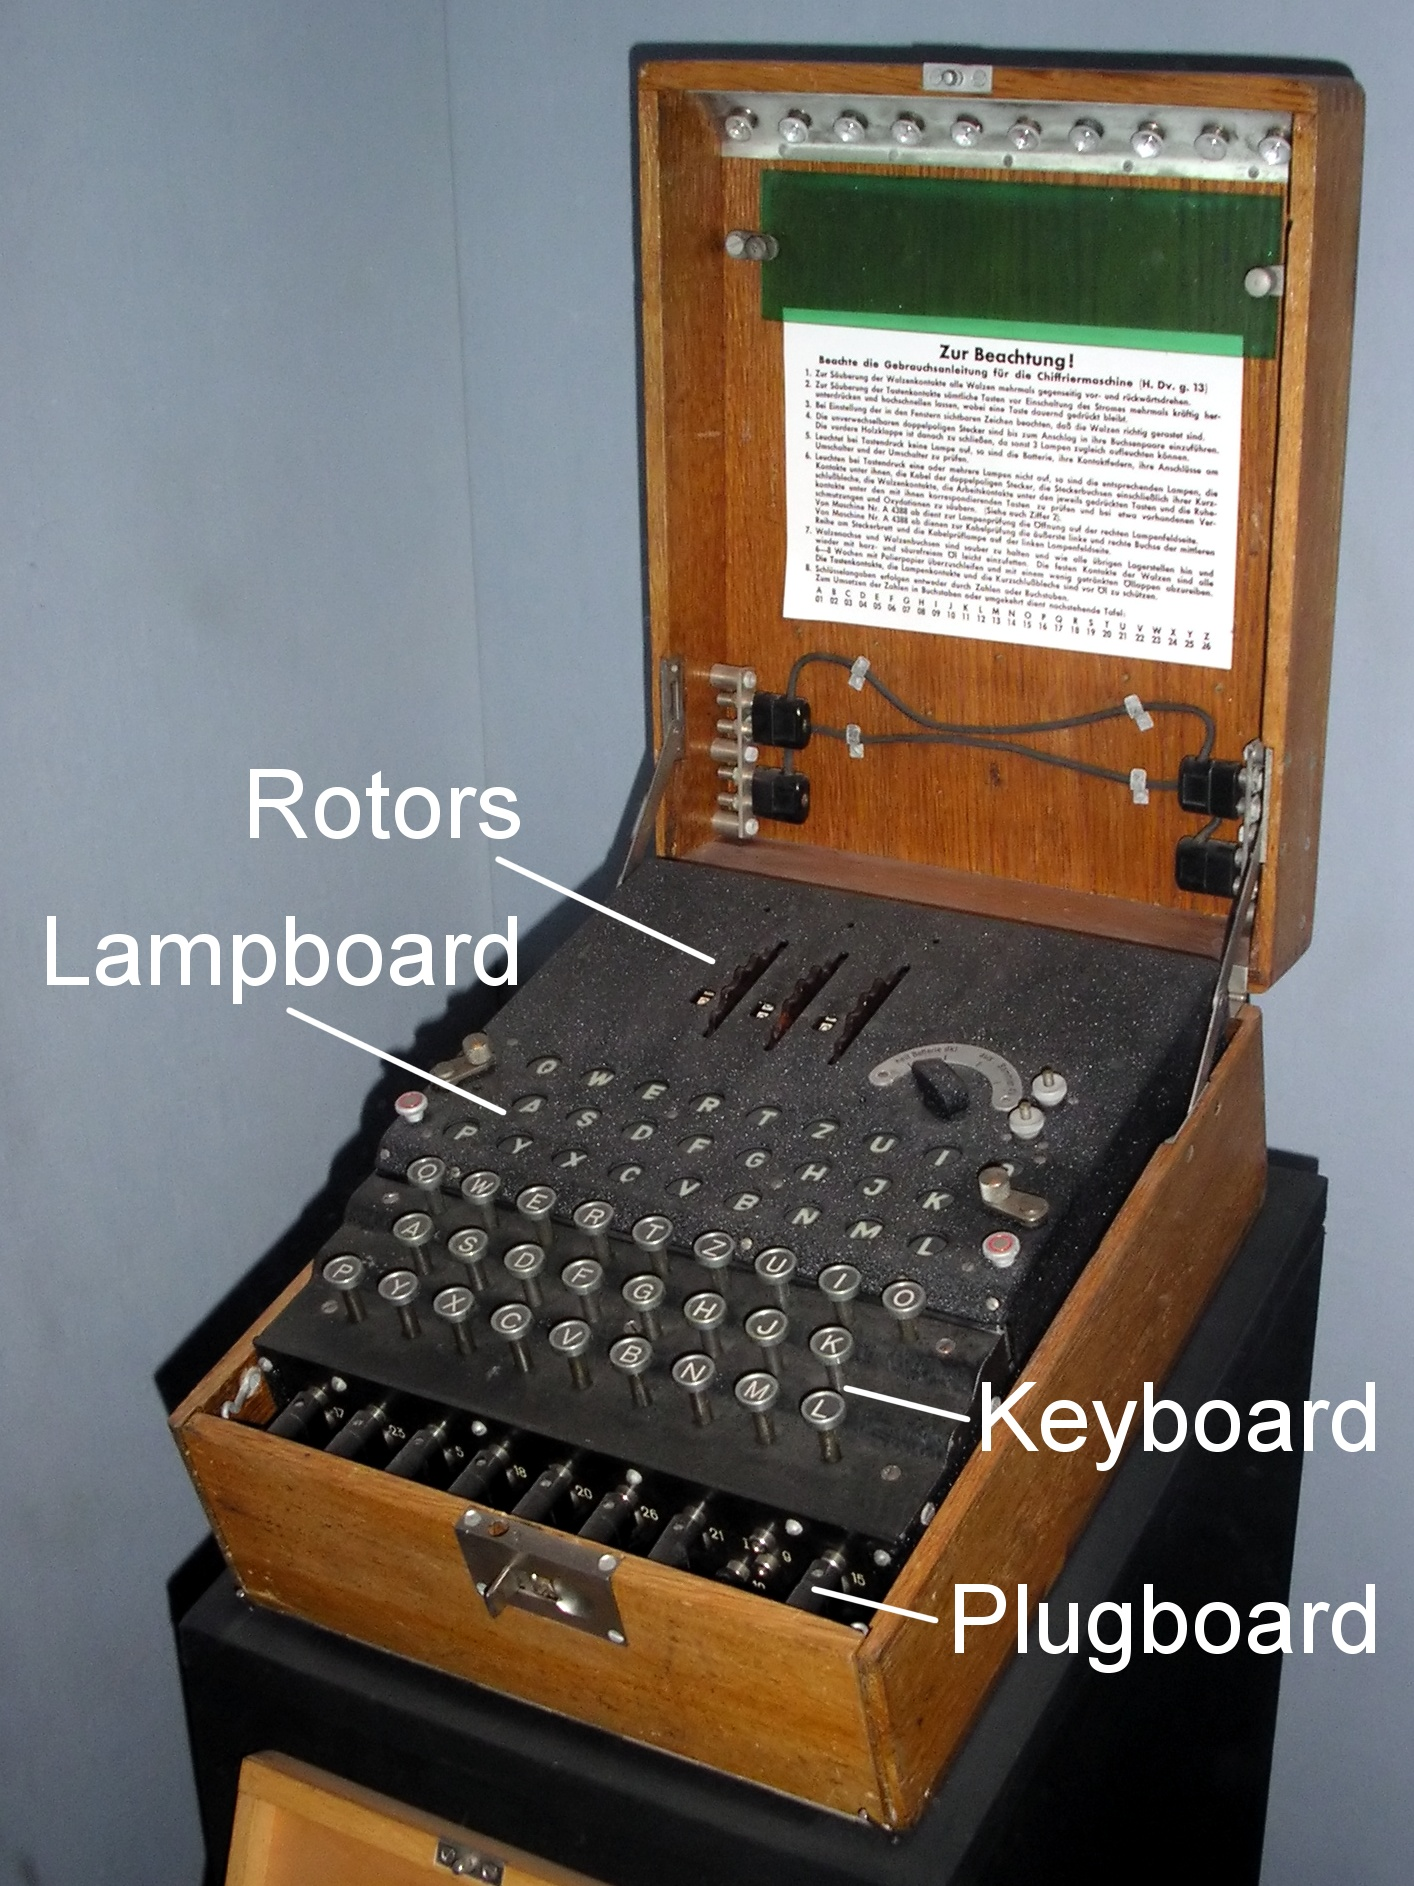
\includegraphics[width=0.5\textwidth]{../img/machine}
	\caption{Enigma Machine - Military Edition}
	\label{fig:machine}
\end{figure}

In the military version of the Enigma Machine there were 5 possible rotors to pick from, each with 26 possible positions, then there were 10 possible switching in the plugboard that could choose a pair from the available 26 letters. That accounts for $158962555217826360000$ different combinations for
the setting of the army Enigma Machine \cite{numberphile1}. The initial setting for each day was given to the bases in a sheet of paper that had the monthly configurations of the machine. So they changed the setting everyday. \\

So in order to decipher the code, you needed either to have the code sheet or to break the message. This latter was what the scientists at Bletchley Park did; and what I will try to recreate in this project. 

\section{General Goal}

To understand the code breaking process behind the enigma cipher.


\section{Specific Goals}

\begin{itemize}
	\item To implement the Enigma machine with software
	\item To implement the Bombe machine that breaks the Enigma cipher
	\item To understand the mathematical and probabilistic techniques used to break a cipher with limited time and computational resources. 
	\item To understand the weaknesses exploited that allowed to break the Enigma cipher
\end{itemize}


\section{Implementation}

I implemented a project in the Python programming language that replicates both the Enigma Machine and the Bombe Machine. I explain in the following subsections the details of each of them.

\subsection{Enigma Machine}

There are different models of the Enigma machine that were developed through time. In this project I chose one of the latest, i.e. with more complicated settings. This is the model M3 \& M4 Naval (from Frebuary 1942) that has 8 possible rotors \cite{dade,wikirotors}. 

\subsubsection{Enigma's algorithm}
The enigma machine consists on a set of physical connections that allow electrical signals to travel through inner cross wirings that move place every time a key is pressed. In the most simple form we could express that any typed key in the keyboard is transformed to another letter that lights up in the bulbs panel. So we could say: 

$$\rm{SIGNAL_{OUT}} = P( S ( P(\rm{SIGNAL_{IN}}) ) )$$

$$S(\rm{SIGNAL}) = R_1(R_2(R_3(F(R_3(R_2(R_1(\rm{SIGNAL})))))))$$

Where $P$ represents the Plugboard; $S$ represents the Set of rotors an reflectors; $R_i$ represents the i-th rotor (in this case there are 3 but there could be more); and $F$ represents the reflector. All of this process can be graphically understood with the image below (Fig. \ref{fig:wiring}): 

\begin{figure}[h!]
	\centering
	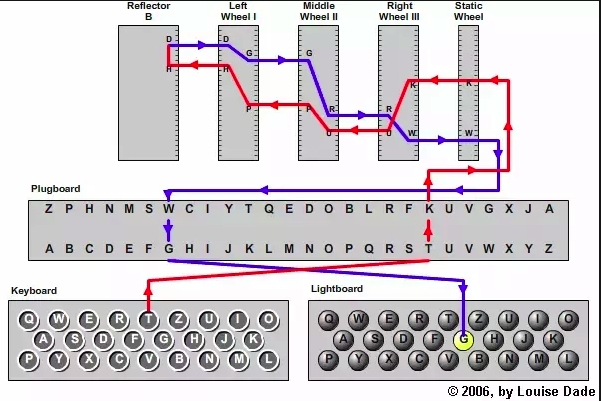
\includegraphics[width=0.55\textwidth]{../img/wiring_example}
	\caption{Enigma Machine Wiring}
	\label{fig:wiring}
\end{figure}

The machine has a symmetric property so in order to decipher the message one has to put the same rotor settings as when the person typing the message started. So this leads us to the configuration of the machine, i.e. the input. 

\subsubsection{Input}
The machine has different settings that changed each day and that were communicated via code sheets like the one in Fig. \ref{fig:code_sheet}. 

\begin{figure}[h!]
	\centering
	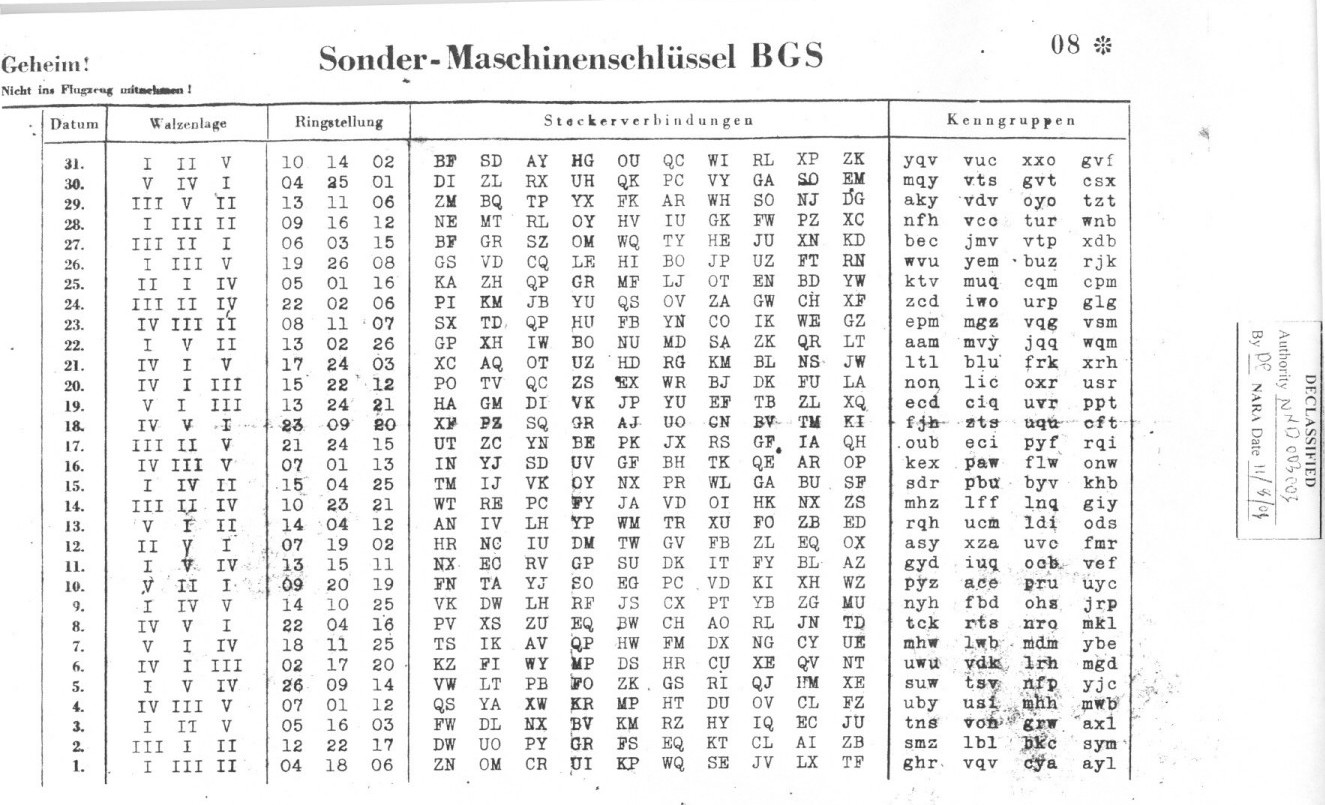
\includegraphics[width=\textwidth]{../img/code_sheet_example}
	\caption{Enigma Machine Wiring}
	\label{fig:code_sheet}
\end{figure}

I handle this as a configuration text file in my implementation. I will describe the components as follows: 

\begin{itemize}
	\item Rotor selection and order: Depending on the machine there are up to 8 different rotors (I-VIII) from which to choose 3 or 4. So an input is which of them and in which permutation from left to right. Example - V IV I.
	\item Rotor's ring settings (\textit{Ringstellung}): Within each rotor there is an internal ring that maps position to a letter, but it can be switched so that the internal wiring mapping is offset. Example - N D V.
	\item Rotor's initial positions (\textit{Grundstellung}): Within the machine, when locating the rotors, they have to be in a particular initial position. This is achieved by inserting the rotor and turning it to the respective starting point. Example: D Y A.
	\item Plugboard pairs: This corresponds to the symmetric correspondence of letters in the other plugboard panel. They are typically 10 pairs. 
	\item Reflector selection: As with the rotors, there are 4 different reflectors from which to choose, all with different cross-connections. 
\end{itemize}

Apart from all of these values that changes from user to user, I also have an input configuration file that loads the historically accurate wiring of each reflector and rotor. For the rotors there is an additional parameter called the turnover point. The rotors work as a clock in the way they rotate. The right-most represent the second, the middle the minutes, and the left-most the hours. However they don't turn all in the same letter ('Z' as one would expect), they all each have their own turnover point that triggers its right partner rotation. Those turnovers are obtained from \cite{wiki}. Finally the message to cipher is also input as a text file. \\

\subsubsection{Processing}
As for the processing of the plain text, here is a pseudo code with the simplified process:

\begin{lstlisting}[language=Python]

for letter in text:

	# advance rotors according to their own position,
	# and turnover points
	step_rotors()
	
	# enter plugboard switch, if no correspondance there 
	# is no connection, so letter doesn't change
	plugboard_letter = plugboard.get(letter, letter)
	
	# enter rotors (inwards - right to left)
	rotor_names_inverted = rotor_names[::-1]
	pin_in = ALPHABET.index(plugboard_letter)
	
	for rotor_name in rotor_names_inverted:
		rotor = rotors[rotor_name]
		pin_in = rotor.process_inwards(pin_in)
	
	# enter reflector
	pin_out = reflector.reflect(pin_in)
	
	# enter rotors (outwards - left to right)
	for rotor_name in rotor_names:
		rotor = rotors[rotor_name]
		pin_out = rotor.process_outwards(pin_out)
	
	# enter plugboard switch
	rotor_letter = ALPHABET[pin_out]
	
	# calculate ciphered letter
	ciphered_letter = plugboard.get(rotor_letter, rotor_letter)
	
\end{lstlisting}

Somethings to be aware of in the processing are that the rotors step before ciphering, not after. Also, the turnover points need to be checked each time the rotors step, some of them  even have 2 different turnovers. 

\subsubsection{Output}
The output of the machine is straightforward, it correspond to the cipher letter of each key press after going through the transformations. And for a whole text is just the concatenation of those letters. If this output is to be typed again in the machine with the same initial configuration, the operator on the other side of the line will obtain the original plain message. \\

\subsubsection{Challenges}

The biggest challenge in implementing the Enigma machine is knowing exactly how it worked. Even thought there is a great amount of information online, the depth of it is not that significant. Most of the resources tend to shallowly explain the behavior but there are several subtleties and details that were hard to find. I put in the references the most trustworthy and complete information I found on the matter \cite{rijmenants,sale,cryptomuseum,wiki,wikicryptanalysis,ellsbury}. \\

Another challenge was the translation of this information, because the original machine settings are in German. This implies that there are multiple acceptable translations for several parts of the machine that might be opposite among different sources. A concrete example of this goes within the rotor, where there are 2 different settings called \textit{Ringstellung} and \textit{Grundstellung}. They refer to the ring setting within each the rotor and to the ground setting or offset of the rotor within the machine, respectively. However figuring out which one was which presented a problem because different sources referred to them by different names, sometimes even opposite. So I had to solve this by recurring to the German words. \\

Finally, I would like to refer as well to different simulators that are found on the internet in which I could get a phenomenological understanding of the machine. I was able to try out different configurations and learning its way to function. I also confirmed my solution against these simulators in order to test my implementation. This was a positive match. 

\begin{itemize}
	\item Cryptii Simulator: \url{https://cryptii.com/pipes/enigma-machine}
	\item Louise Dade Simulator: \url{http://enigma.louisedade.co.uk/enigma.html}
\end{itemize}



\subsection{Bombe Machine}

\subsubsection{Enigma Exploits}

In order to break the enigma, mathematicians Alan Turing and Gordon Welchman, with the collaboration of the staff at Bletchley Park, design the Bombe Machine. It exploited the Enigma Machine's flaws to crack the Nazi's communications. However, the machine itself was not all, it exploited behavioral patterns in the communication as well. Here I list the main weaknesses that lead to deciphering the Enigma:

\begin{itemize}
	\item The biggest flaw of the Enigma Machine is that because of the internal wiring and design, a letter can never be encrypted to itself. This opened the door to cryptoanalysts to locate possible message deciphers. \cite{numberphile2}
	\item Another breakthrough was when they realized about specific patterns that would repeat themselves in a conversation. For example the daily weather forecast, the heil Hitler salute, or war jargon. These parts of the conversation tipically followed a standard format that allows to create "cribs", an intelligent guess of part of the code. \cite{computerphile}
	% ex: "weather for the night" "situation eastern channel" "beacons lit as ordered" etc
	\item In addition to the previous facts, sometimes reckless operators forgot to change the daily settings, which lower the odds of combinations and gave more data to the analysts.
	
\end{itemize}

\subsubsection{Bombe's algorithm}

- with those typical messages we can scan the transmissions and locate where it is within the text (where no letter ciphers to itself)

- with all the possible positions we create a set of hypothesis called a menu, a diagram like fig x. from there, we need to fing a enigma configuration that corresponds to the menu. that was the role of the bombe https://www.youtube.com/watch?v=2dKG21u2aSo

\subsubsection{Input}

\subsubsection{Processing}

\subsubsection{Output}

\subsubsection{Challenges}

-getting info, very sensitive, most of it classified. Some of it released in 2010, less than 10 years ago
-less than 200 bombes, as opposed to enigma machines that were even commercial

...

Finally, and as in the previous step, I got some insights from two Bombe simulators online. However as the is very complex, using them is not as straightforward and required a lot of learning. After all, each bomb had several operators. So I just had a glimpse on their configuration files, specially the menu input. Here are the references: 

\begin{itemize}
	\item Ekhall \& Hallenberg Simulator: \url{http://www.lysator.liu.se/~koma/turingbombe/} \cite{ekhall}
	\item 101 Computing Simulator: \url{https://www.101computing.net/turing-welchman-bombe/}
\end{itemize}


\subsection{Code}
The code of both machines is available in the project attached to this report. The structure is as follows: 

PICTURE OF CODE STRUCTURE

There is a program called \texttt{example.py} that shows how to use the programs and when executed, outputs the result of both enigma and bombe machines to their respective results files. It also outputs to console like this: 

\begin{figure}[h!]
	\centering
	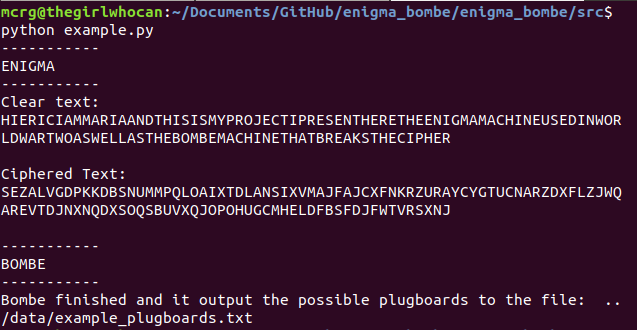
\includegraphics[width=0.8\textwidth]{../img/code_stdout}
	\caption{Example Code Standard Output}
	\label{fig:code_stdout}
\end{figure}


\section{Discussion}

- historic relevance
- not only breaking it, it needed strategy, not letting them know they cracked the code
- conclusions, goals achieved

\subsection{Future Work}



\begin{thebibliography}{10}
% -- enigma --
	\bibitem{hodges} A. Hodges. \textit{Alan Turing: The Enigma}. Princeton, N.J: Princeton University Press (2012). 
	\bibitem{numberphile1} Numberphile. \textit{158,962,555,217,826,360,000 (Enigma Machine)}. YouTube (2013). % https://www.youtube.com/watch?v=G2_Q9FoD-oQ
	\bibitem{rijmenants} D. Rijmenants. \textit{Technical Details of the Enigma Machine}. Obtained from: \url{http://users.telenet.be/d.rijmenants/en/enigmatech.htm}
	\bibitem{sale} T. Sale. \textit{Military Use of the Enigma}. Obtained from: \url{https://www.codesandciphers.org.uk/enigma/enigma3.htm}
	\bibitem{cryptomuseum} Cryptomuseum. \textit{Enigma Cipher Machines}. Obtained from: \url{https://www.cryptomuseum.com/crypto/enigma/index.htm}	
	\bibitem{wiki} Wikipedia. \textit{Enigma Machine}. Obtained from: \url{https://en.wikipedia.org/wiki/Enigma_machine}
	\bibitem{wikicryptanalysis} Wikipedia. \textit{Cryptanalysis of the Enigma}. Obtained from: \url{https://en.wikipedia.org/wiki/Cryptanalysis_of_the_Enigma}
	
	\bibitem{dade} L. Dade. \textit{Enigma Machine: How It Works}. Obtained from: \url{http://enigma.louisedade.co.uk/howitworks.html}
	\bibitem{wikirotors} Wikipedia. \textit{Enigma Rotor Details}. Obtained from: \url{https://en.wikipedia.org/wiki/Enigma_rotor_details}
	
% -- bombe --
	\bibitem{ellsbury} G. Ellsbury. \textit{The Enigma and The Bombe}. Obtained from: \url{http://www.ellsbury.com/enigmabombe.htm}
	\bibitem{numberphile2} Numberphile. \textit{Flaw in the Enigma Code}. YouTube (2013). % https://www.youtube.com/watch?v=V4V2bpZlqx8
	\bibitem{computerphile} Computerphile. \textit{Tackling Enigma (Turing's Enigma Problem)}. YouTube (2013). % https://www.youtube.com/watch?v=kj_7Jc1mS9k
	\bibitem{ekhall} M. Ekhall, F. Hallenberg. \textit{US Navy Cryptanalytic Bombe - A Theory of Operation and Computer Simulation}. Proceedings of the 1st Conference on Historical Cryptology, pages 103-108,	Uppsala, Sweden, 18-20 June, 2018.
	
	
	
\end{thebibliography}


\end{document} 